\documentclass{desyproc}

\begin{document}
%------------------------------------
\title{RooUnfold --- unfolding framework and algorithms}

\author{{\slshape Tim Adye$^1$, Kerstin Tackmann$^2$, Fergus Wilson$^1$}\\[1ex]
$^1$Rutherford Appleton Laboratory, Science and Technology Facilities Council, Harwell Science and Innovation Campus, Didcot OX11 0QX, United Kingdom\\
$^2$CERN, CH-1211 Geneva 23, Switzerland}

% please do not modify the following 5 lines
\contribID{xy}  % will be entered by the editors
\confID{3009}
\desyproc{DESY-PROC-2010-02}
\acronym{Unfolding 2010}
\doi            % will be entered by the editors

\maketitle

\begin{abstract}
\end{abstract}

\section{RooUnfold package aims and features}

The RooUnfold package~\cite{RooUnfold-web} was designed to provide a framework for different unfolding algorithms.
This approach simplifies the comparison between algorithms and has allowed
common utilities to be written.

Currently RooUnfold implements the iterative Bayes~\cite{D'Agostini:1994zf},
Singular Value Decomposition (SVD)~\cite{Hocker:1995kb}, and correction factors methods.
In these cases RooUnfold was interfaced to existing code, which
was then adapted and improved in-situ. We plan to continue this process with
other algorithms.

The package is designed around a simple object-oriented approach, implemented in
C++, and using existing ROOT~\cite{Brun:1997pa} classes. RooUnfold defines classes for the different
unfolding algorithms, which inherit from a common base class, and a class for
the response matrix. The response matrix object is independent of the unfolding,
so can be filled in a separate ``training'' program.

RooUnfold can be linked into a stand-alone program, run from a ROOT/CINT script, or
executed interactively from the ROOT prompt.
The response matrix can be initialised using existing histograms or matrices, or
filled with build-in methods (these can take care of the normalisation when inefficiencies are to be considered).
The results can be returned as a histogram with errors, or a vector with full covariance matrix.

The framework also takes care of handling multi-dimensional distributions
(with ROOT support for 1--, 2--, and 3--dimensional histograms),
different binning for measured and truth distributions,
variable binning, and the option to include or exclude of under- and over-flows.
These details are handled by the framework, so don't have to be
implemented for each algorithm. However different bin layouts may not produce good results for
algorithms that rely on the global shape of the distribution (SVD).

Common utility routines are provided for displaying the results with resolutions,
pulls, and $\chi^2$. A toy Monte Carlo (MC) test framework is also provided, allowing
selection of different MC probability distribution functions (PDF) and parameters,
comparing different binning, and performing the unfolding with the different
algorithms and varying the unfolding regularisation parameters.
Tests can be performed with 1D, 2D, and 3D distributions.
A few example tests are presented in section~\ref{sec:adye:examples}.



\section{C++ classes}

\begin{figure}[hb]
\centerline{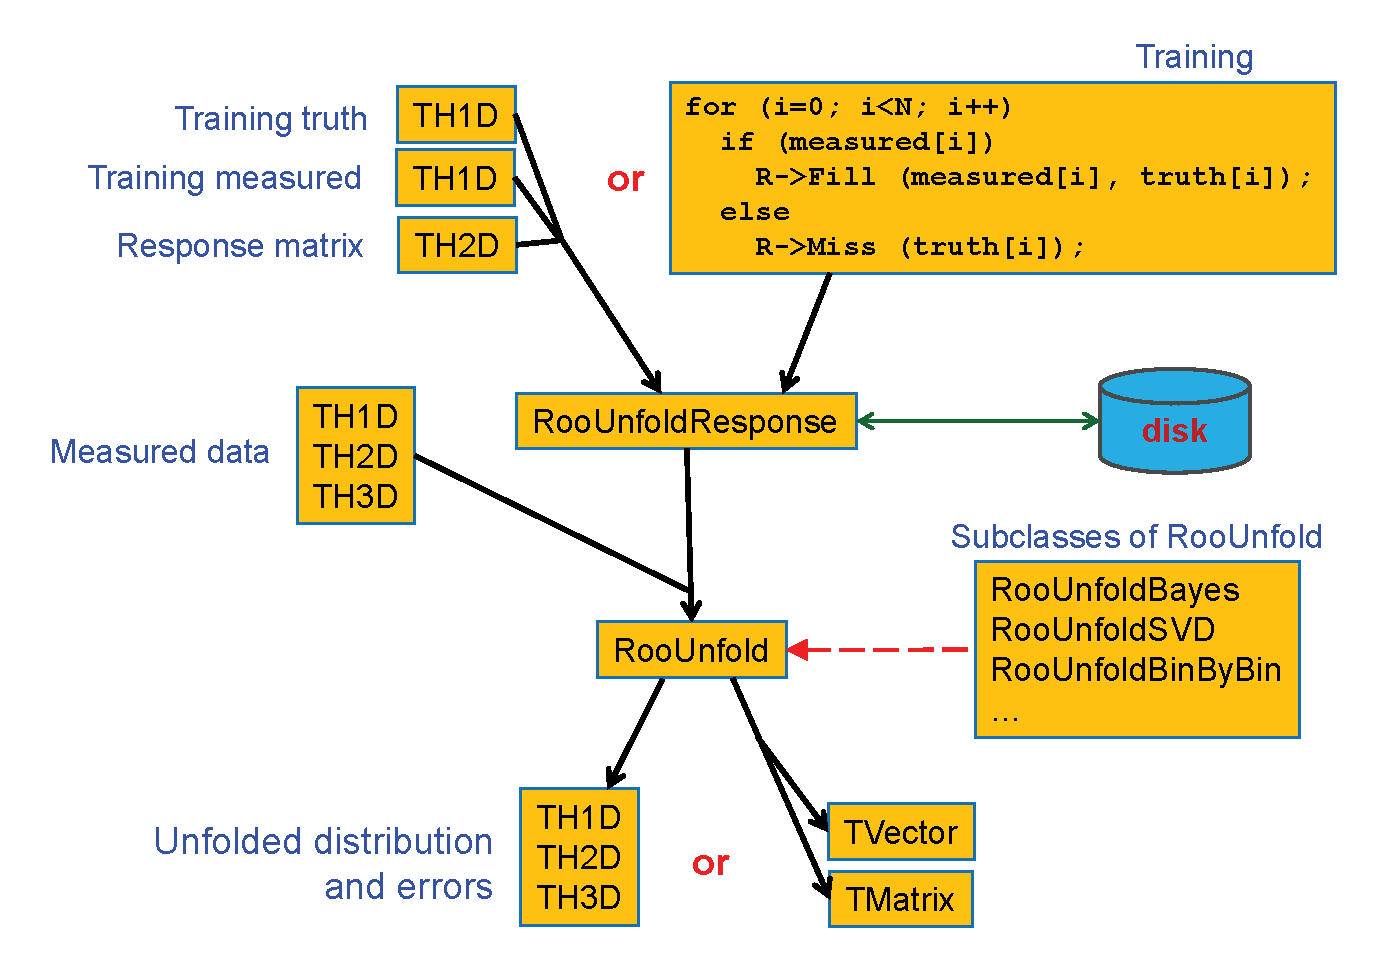
\includegraphics[width=\textwidth]{adye_tim.classes.eps}}
\caption{RooUnfold classes}\label{Fig:adye:classes}
\end{figure}

Figure~\ref{Fig:adye:classes} summarises how the ROOT and RooUnfold classes are used
together. The RooUnfoldResponse object can be constructed using a 2D response histogram (TH2D)
and 1D truth and measured projections (these are required to determine the effect of inefficiencies).
Alternatively, RooUnfoldResponse can be filled directly with the

\begin{quote}
\texttt{response->Fill($x_{\rm measured}$, $x_{\rm true}$)}
\end{quote}

and

\begin{quote}
\texttt{response->Miss($x_{\rm true}$)}
\end{quote}

methods, where the \texttt{Miss} method is used to count an event that was not measured
and should be counted towards the inefficiency.

The RooUnfoldResponse object can be saved to disk using the usual ROOT input/output
streamers. This allows the easy separation in separate programs
of MC training from the unfolding step.

A RooUnfold object is constructed using a RooUnfoldResponse object and the measured
data. It can be constructed as a RooUnfoldBayes, RooUnfoldSVD, or RooUnfoldBinByBin
object, depending on the algorithm required.

The results of the unfolding can be obtained as ROOT histograms (TH1D, TH2D, or TH3D)
or as a ROOT vector (TVectorD) and covariance matrix (TMatrixD). The histogram will
include just the diagonal elements of the error matrix, which may be misleading
given the significant correlations that can occur if there is much bin-to-bin migration.

\section{Unfolding algorithms}

\subsection{Iterative Bayes' theorem}

The RooUnfoldBayes algorithm uses the method described by Giulio D'Agostini in~\cite{D'Agostini:1994zf}.

Repeated application of Bayes' theorem is used to invert the response matrix.
Regularisation is achieved by stopping iterations before reaching ``true''
(but wildly fluctuating) inverse.
The regularisation parameter is just the number of iterations.
In principle, this has to be tuned according to the sample statistics and binning.
In practice, the results are fairly insensitive to the precise setting used.

RooUnfoldBayes takes the training truth as its initial prior, rather than a flat distribution,
as described by D'Agostini.
This should not bias result once we have iterated, but could reach an optimum after fewer iterations.

This implementation takes account of multinomial errors on the data sample but not,
by default, uncertainties in the response matrix due to finite MC statistics.
That calculation can be very slow, and usually the training sample is much larger
than the data sample.

RooUnfoldBayes does not normally do smoothing, since this has not been found to be necessary
and can, in principle, bias the distribution. Smoothing can be enabled with an option.

\subsection{Singular Value Decomposition}

RooUnfoldSVD uses the method of Andreas H\"ocker and Vakhtang Kartvelishvili~\cite{Hocker:1995kb}
and originally implemented for the BaBar $B \rightarrow X_ul\nu$ measurement~\cite{Aubert:2004bq}.

The response matrix is inverted using singular value decomposition.
(The normalisation to the number of events is retained in order to keep
track of the MC uncertainties.)
Regularisation is performed using a smooth cut-off on small singular value contributions
(these correspond to high-frequency fluctuations) by replacing
$s_i^2 \rightarrow s_i^2 / (s_i^2 + s_k^2)$ where the choice of cut-off singular value index, $k$,
determines the relative contributions of MC truth and data.

If $k$ is too small, the result is dominated by MC truth. 
If $k$ is too large, the result is dominated by statistical fluctuations.
$k$ needs to be tuned for the particular type of distribution, number of bins, and approximate sample size.

The unfolded error matrix includes the contribution of uncertainties on the
response matrix due to finite MC training statistics, though these are usually quite small.

\subsection{Simple correction factors}

A very simple algorithm using bin-by-bin correction factors,
with no inter-bin migration is included to aid comparison.

\section{Examples\label{sec:adye:examples}}

Examples of toy MC tests generated by RooUnfoldTest are shown in Figures~\ref{Fig:adye:training-example}--\ref{Fig:adye:svd-example}.

\begin{figure}[ht]
\centerline{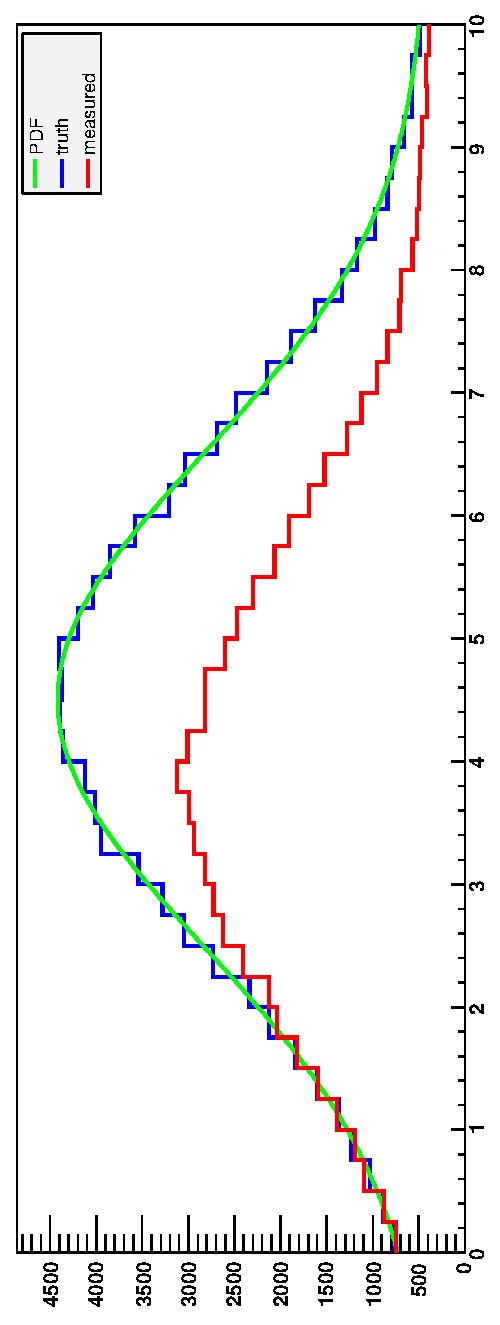
\includegraphics[angle=-90,width=0.92\textwidth,clip]{adye_tim.bayes1.eps}}
\caption{Example of a toy MC training run.
A Gaussian PDF on a flat background (green curve) is used to generate
a training ``truth'' sample (upper histogram in blue). This is then smeared, shifted,
and a variable inefficiency applied to produce the ``measured'' distribution
(lower histogram in red).
}\label{Fig:adye:training-example}
\end{figure}%
\begin{figure}[ht]
\centerline{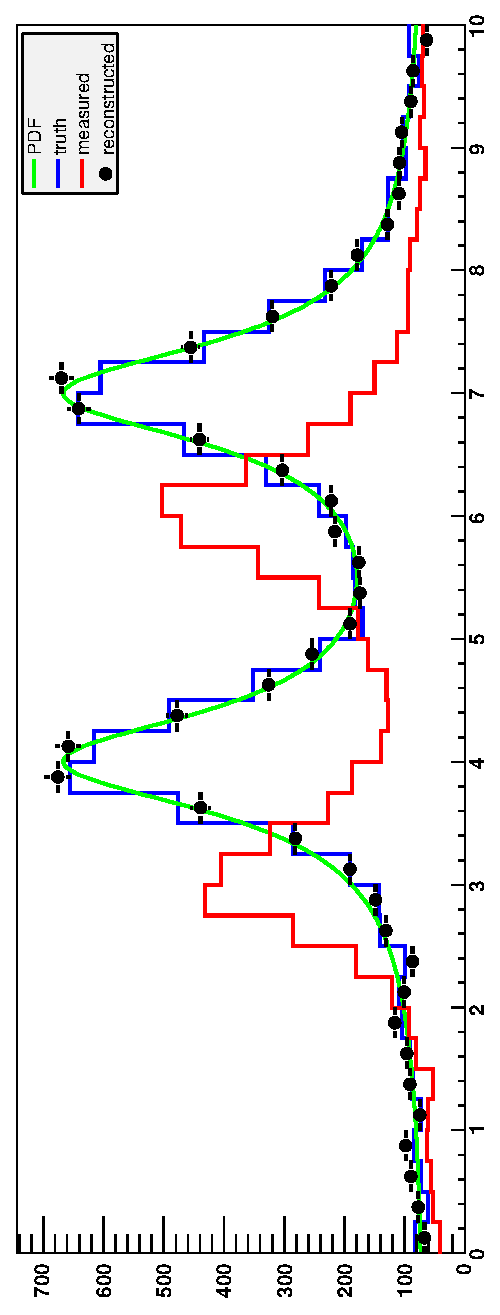
\includegraphics[angle=-90,width=0.92\textwidth,clip]{adye_tim.bayes2.eps}}
\caption{Unfolding with the Bayes algorithm.
A double Breit-Wigner PDF on a flat background (green curve) is used to generate
a training ``truth'' sample (upper histogram in blue). The same resolution effects
as were used in training (Figure~\ref{Fig:adye:training-example}) were applied
to produce the ``measured'' distribution (lower histogram in red).
Applying the Bayes algorithm with 3~iterations on this latter gave the unfolded result
(black points), shown with errors from the diagonal elements of the error matrix.
}\label{Fig:adye:bayes-example}
\end{figure}%
\begin{figure}[ht]
\centerline{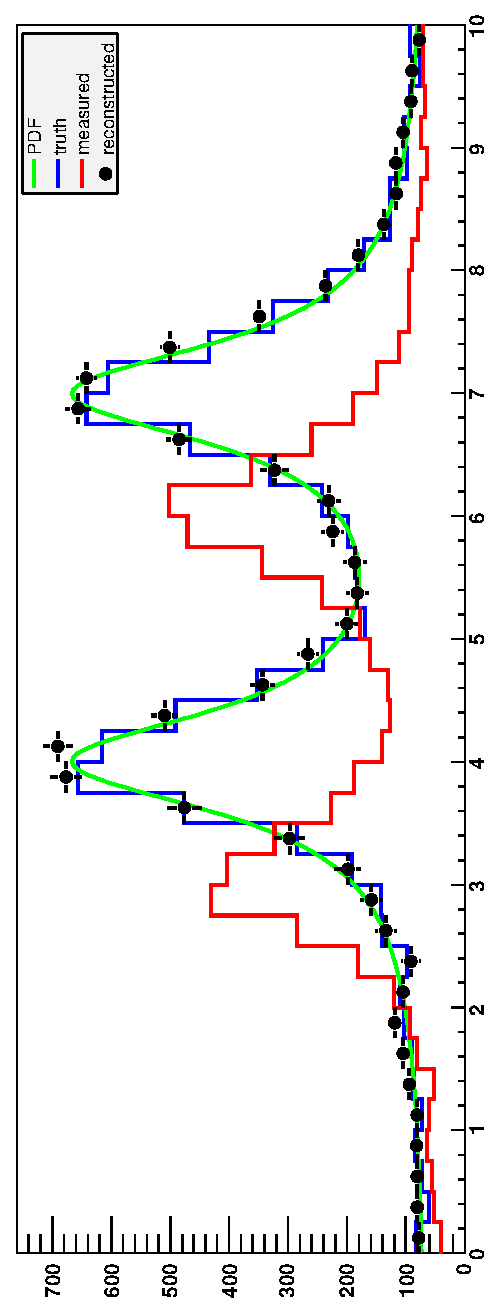
\includegraphics[angle=-90,width=0.92\textwidth,clip]{adye_tim.svd2.eps}}
\caption{Unfolding with the SVD algorithm ($k=20$) on
the same training and test samples as described in Figures~\ref{Fig:adye:training-example}
and~\ref{Fig:adye:bayes-example}.}\label{Fig:adye:svd-example}
\end{figure}

\section{Status and Plans}

RooUnfold was first developed in the BaBar software environment.
It was released stand-alone in 2007.
Since then, it has been used by physicists from many
different particle physics, particle-astrophysics, and nuclear physics groups.
Questions, suggestions, and even a few bug reports from users
have prompted new versions with fixes and improvements.

We plan further improvements, namely to

\begin{itemize}

\item provide additional input/output methods (eg. RooFit~\cite{Verkerke:2003ir} datasets);

\item add common tools, useful for all algorithms, such as 
automating the validation and selection of regularisation parameters;

\item interface with additional algorithms; and

\item publish RooUnfold as an official ROOT package as part of the RooStats collection~\cite{RooStats}.
\end{itemize}

% ****************************************************************************
% BIBLIOGRAPHY AREA
% ****************************************************************************

% please do not change the following line
\begin{footnotesize}

\begin{thebibliography}{99}

\bibitem{RooUnfold-web}
  The RooUnfold package and documentation are available from\\
  \verb=http://hepunx.rl.ac.uk/~adye/software/unfold/RooUnfold.html=

\bibitem{D'Agostini:1994zf}
  G.~D'Agostini,
  ``A Multidimensional unfolding method based on Bayes' theorem,''
  Nucl.\ Instrum.\ Meth.\  A {\bf 362} (1995) 487.
  %%CITATION = NUIMA,A362,487;%%

\bibitem{Hocker:1995kb}
  A.~Hocker and V.~Kartvelishvili,
  ``SVD Approach to Data Unfolding,''
  Nucl.\ Instrum.\ Meth.\  A {\bf 372} (1996) 469
  [arXiv:hep-ph/9509307].
  %%CITATION = NUIMA,A372,469;%%

\bibitem{Brun:1997pa}
  R.~Brun and F.~Rademakers,
  ``ROOT: An object oriented data analysis framework,''
  Nucl.\ Instrum.\ Meth.\  A {\bf 389} (1997) 81.
  %%CITATION = NUIMA,A389,81;%%
  See also \verb=http://root.cern.ch/=.

\bibitem{Aubert:2004bq}
  B.~Aubert {\it et al.}  [BABAR Collaboration],
  ``Study of $B \to u \ell \bar{\nu}$ decays on the recoil of fully reconstructed $B$ mesons and determination of $|V_{ub}|$,''
  arXiv:hep-ex/0408068.
  %%CITATION = HEP-EX/0408068;%%

\bibitem{Verkerke:2003ir}
  W.~Verkerke and D.~P.~Kirkby,
  ``The RooFit toolkit for data modeling,''
  %{\it In the Proceedings of 2003 Conference for Computing in High-Energy and Nuclear Physics (CHEP 03), La Jolla, California, 24-28 Mar 2003, pp MOLT007}
  arXiv:physics/0306116.
  %%CITATION = ECONF,C0303241,MOLT007;%%

\bibitem{RooStats}
  RooStats Wiki,
  \verb=https://twiki.cern.ch/twiki/bin/view/RooStats/WebHome=

\end{thebibliography}

% please do not change the following line
\end{footnotesize}

% ****************************************************************************
% END OF BIBLIOGRAPHY AREA
% ****************************************************************************

\end{document}
